\chapter{Software Design}

\section{Introduction to Software Design}

This chapter presents the detailed software design of the TechAware AI-Based Feedback System. It translates the requirements identified in Chapter 3 into structured architectural, behavioral, and data models. The purpose of this chapter is to provide a clear blueprint for system implementation, ensuring maintainability, scalability, and modular development.

This chapter includes architectural design, UML models, data flow models, and database design applicable to the web-based feedback management system.

%%%%%%%%%%%%%%%%%%%%%%%%%%%%%%%%%%%%%%%%%%%%%%%%%%%%%%
\section{Design Methodology and Software Process Model}

\subsection{Design Methodology}

This project follows a Layered Architecture design methodology combined with Object-Oriented Design (OOD) principles. The system is organized into three distinct layers:

\begin{itemize}
    \item Presentation Layer (HTML/CSS/JavaScript templates)
    \item Application Layer (Flask backend with business logic and NLP processing)
    \item Data Layer (SQLAlchemy ORM with SQLite database)
\end{itemize}

The selected methodology ensures modularity, loose coupling, reusability, and scalability. The layered approach was chosen because the web-based nature of the system requires clear separation between user interface rendering, business logic processing (including sentiment analysis), and data persistence. Design principles followed include Separation of Concerns, DRY (Don't Repeat Yourself), and modular code organization with separate files for models, database initialization, and application routes.

%%%%%%%%%%%%%%%%%%%%%%%%%%%%%%%%%%%%%%%%%%%%%%%%%%%%%%
\subsection{Software Process Model}

The project follows the \textbf{Agile} model with iterative development cycles. The Agile approach was selected due to the evolving nature of feedback system requirements and the need for continuous stakeholder feedback during development.

Development was organized into six iterative phases: Core Infrastructure (database and models), Academic Management (departments, batches, sections, courses), Timetable and Attendance System, Feedback Collection and Sentiment Analysis, Portal Development and Analytics, and Enhancements (email notifications, reporting, security). Each iteration included requirement refinement, implementation, and testing, ensuring that functional components were delivered incrementally and validated before proceeding to the next phase.

%%%%%%%%%%%%%%%%%%%%%%%%%%%%%%%%%%%%%%%%%%%%%%%%%%%%%%
\section{System Overview}

This section provides a high-level overview of the TechAware system components and their interactions with external entities. The context diagram below illustrates the system boundary, identifying external actors (Student, Teacher, Administrator, Batch Advisor) and external systems (Gmail SMTP, Chart.js CDN) that interact with the application.

\begin{figure}[H]
\centering
\resizebox{0.9\textwidth}{!}{%
\begin{tikzpicture}[node distance=1.5cm and 2cm, every node/.style={font=\small, text width=2.8cm, align=center}]
    % External entities (sharp squares)
    \node[draw, rectangle, minimum width=2.6cm] (student) {Student};
    \node[draw, rectangle, right=of student, minimum width=2.6cm] (teacher) {Teacher};
    \node[draw, rectangle, right=of teacher, minimum width=2.6cm] (admin) {Administrator};
    \node[draw, rectangle, right=of admin, minimum width=2.6cm] (advisor) {Batch Advisor};

    % System boundary
    \node[draw, rectangle, rounded corners, minimum width=13cm, minimum height=4cm, below=1.2cm of teacher] (sys) {\textbf{TechAware Feedback System}};

    % Core processes inside system
    \node[draw, rounded corners, below left=0.4cm and 2.6cm of sys] (collect) {Feedback Collection};
    \node[draw, rounded corners, below=0.4cm of sys] (analysis) {Sentiment Analysis};
    \node[draw, rounded corners, below right=0.4cm and 2.6cm of sys] (dashboard) {Dashboard / Reporting};

    % Data store (parallel lines)
    \node[draw, rectangle, minimum width=2.6cm, minimum height=1.0cm, below=of analysis] (db) {Feedback Database};
    \draw ($(db.north west)+(0.12,-0.12)$) -- ($(db.south west)+(0.12,0.12)$);
    \draw ($(db.north west)+(0.30,-0.12)$) -- ($(db.south west)+(0.30,0.12)$);

    % Flows
    \draw[->] (student) -- ++(0,-0.6) -| (collect.north) node[midway, right, font=\footnotesize]{feedback(session,data)};
    \draw[->] (collect) -- (analysis) node[midway, right, font=\footnotesize]{text,rating};
    \draw[->] (analysis) -- (db) node[midway, right, font=\footnotesize]{polarity, suggestions};
    \draw[->] (db.north) -- ++(0,0.6) -| (dashboard.south) node[midway, above, font=\footnotesize]{records};
    \draw[->] (analysis.east) -- ++(1.2,0) |- (teacher.south) node[midway, right, font=\footnotesize]{alerts}
        ;
\end{tikzpicture}%
}
\caption{Context Diagram of TechAware AI-Based Feedback System}
\label{fig:context}
\end{figure}

The context diagram shows the system as a central process with data flows to and from four actor types and two external services. Students provide feedback data; the system returns sentiment analysis results. Teachers receive feedback analytics and AI suggestions. Administrators manage all system entities. The system communicates with Gmail SMTP for email delivery and retrieves Chart.js from CDN for dashboard visualization.

%%%%%%%%%%%%%%%%%%%%%%%%%%%%%%%%%%%%%%%%%%%%%%%%%%%%%%
\section{Architectural Design}

This section describes the high-level architecture of the TechAware system. The system follows a three-tier web application architecture.

\begin{figure}[H]
\centering
\resizebox{0.9\textwidth}{!}{%
\begin{tikzpicture}[node distance=1.5cm and 2cm, every node/.style={font=\small, text width=2.8cm, align=center}]
    % External entities
    \node[draw, rectangle, minimum width=2.8cm] (smtp) {Gmail SMTP};
    \node[draw, rectangle, right=of smtp, minimum width=2.8cm] (cdn) {Chart.js CDN};

    % System box
    \node[draw, rectangle, rounded corners, minimum width=10cm, minimum height=4cm, right=2.5cm of smtp] (sys) {\textbf{TechAware Feedback System}};

    % Layers inside system
    \node[draw, rectangle, minimum width=8.5cm, minimum height=0.8cm, above=0.5cm of sys] (presentation) {Presentation Layer (HTML/CSS/JS)};
    \node[draw, rectangle, minimum width=8.5cm, minimum height=0.8cm, below=0cm of sys] (application) {Application Layer (Flask Backend)};
    \node[draw, rectangle, minimum width=8.5cm, minimum height=0.8cm, below=0.9cm of application] (data) {Data Layer (SQLite / SQLAlchemy)};

    % Arrows
    \draw[->] (smtp) -- ++(0.6,0) |- (application.west) node[midway, above, font=\footnotesize] {send\_email(payload)};
    \draw[->] (cdn) -- ++(-0.6,0) |- (presentation.east) node[midway, above, font=\footnotesize] {chart.js (assets)};
    \draw[->] (presentation) -- (application) node[midway, right, font=\footnotesize] {AJAX / API calls (JSON)};
    \draw[->] (application) -- (data) node[midway, right, font=\footnotesize] {ORM queries / feedback records};
    \draw[->] (data.west) -- ++(-1.2,0) node[midway, above, font=\footnotesize] {feedback DB};
\end{tikzpicture}%
}
\caption{System Architecture Diagram of TechAware AI-Based Feedback System}
\label{fig:architecture}
\end{figure}

The architecture consists of the following layers:

\begin{itemize}
    \item \textbf{Presentation Layer}: HTML5/CSS3/JavaScript frontend templates rendered by Flask's Jinja2 templating engine. Includes responsive layouts, AJAX-based asynchronous data loading, and Chart.js for data visualization.
    \item \textbf{Application Layer}: Python Flask backend implementing all business logic including user authentication, feedback processing, TextBlob sentiment analysis, AI suggestion generation, SMTP email notification, and ReportLab PDF generation.
    \item \textbf{Data Layer}: SQLAlchemy ORM providing database abstraction over SQLite. Contains 12 interrelated models (User, Department, Batch, Section, Student, Course, Teacher, BatchSubject, CourseTeacher, Feedback, Attendance, Timetable).
\end{itemize}

The interaction between layers follows a request-response pattern: the browser sends HTTP requests to Flask routes, which execute business logic, interact with the database through SQLAlchemy, and return rendered HTML or JSON responses.


%%%%%%%%%%%%%%%%%%%%%%%%%%%%%%%%%%%%%%%%%%%%%%%%%%%%%%
\section{Design Models}

This section presents detailed design models of the system. These models describe system behavior, structure, and interactions using UML diagrams. The models help developers understand system workflow before implementation.

%%%%%%%%%%%%%%%%%%%%%%%%%%%%%%%%%%%%%%%%%%%%%%%%%%%%%%
\subsection{Activity Diagrams}

Activity diagrams represent the workflow of different modules of the system. Each core module has a separate activity diagram illustrating its operational flow.

\begin{figure}[H]
\centering
\resizebox{0.9\textwidth}{!}{%
\begin{tikzpicture}[node distance=1.5cm and 2cm, every node/.style={font=\small, text width=3.2cm, align=center}]
    \tikzstyle{proc}=[draw, rounded corners, minimum width=4cm, minimum height=0.8cm, align=center]
    \node[proc] (start) {Open Feedback Form};
    \node[proc, below=of start] (fill) {Fill Ratings \& Text};
    \node[proc, below=of fill] (validate) {Validate Input};
    \node[proc, below=of validate] (analyze) {Sentiment Analysis (TextBlob)};
    \node[proc, below=of analyze] (store) {Store Feedback (DB)};
    \node[proc, below=of store] (notify) {Send Email Notification};
    \draw[->] (start) -- (fill) ;
    \draw[->] (fill) -- (validate) ;
    \draw[->] (validate) -- node[midway, right, font=\footnotesize]{valid/invalid} (analyze) ;
    \draw[->] (analyze) -- (store) ;
    \draw[->] (store) -- (notify) ;
\end{tikzpicture}%
}
\caption{Activity Diagram -- Student Feedback Submission}
\label{fig:activity}
\end{figure}

%%%%%%%%%%%%%%%%%%%%%%%%%%%%%%%%%%%%%%%%%%%%%%%%%%%%%%
\subsubsection{Module 1: User Authentication}

This diagram illustrates the user login workflow. The process begins when a user enters credentials on the login page. The system validates the email and password against the database. If authentication succeeds, the user is redirected to their role-specific portal (Student Dashboard, Teacher Dashboard, or Admin Panel). If authentication fails, an error message is displayed and the user remains on the login page.

\textbf{Figure 4.4: Activity Diagram -- User Authentication Module}

%%%%%%%%%%%%%%%%%%%%%%%%%%%%%%%%%%%%%%%%%%%%%%%%%%%%%%
\subsubsection{Module 2: Feedback Collection and Analysis}

This diagram illustrates the complete feedback submission and analysis workflow. The student accesses the feedback form, selects the lecture session, provides ratings and text feedback, and submits the form. The system validates inputs, performs sentiment analysis using TextBlob, generates AI suggestions based on keyword matching, stores the feedback in the database, sends an email notification to the teacher, and displays the sentiment result to the student.

\textbf{Figure 4.5: Activity Diagram -- Feedback Collection Module}

%%%%%%%%%%%%%%%%%%%%%%%%%%%%%%%%%%%%%%%%%%%%%%%%%%%%%%
\subsubsection{Module 3: Admin Management Operations}

This diagram illustrates administrative CRUD operations including department creation, batch management, section assignment, course creation, teacher management, and timetable configuration. The admin selects an entity type, performs the desired operation (Create/Read/Update/Delete), the system validates input, updates the database, and displays confirmation.

\textbf{Figure 4.6: Activity Diagram -- Admin Operations}

%%%%%%%%%%%%%%%%%%%%%%%%%%%%%%%%%%%%%%%%%%%%%%%%%%%%%%
\subsection{Class Diagram}

The class diagram shows the static structure of the TechAware system, illustrating all major classes, their attributes, methods, and relationships.

\begin{figure}[H]
\centering
\resizebox{0.9\textwidth}{!}{%
\begin{tikzpicture}[node distance=1.5cm and 2cm, every node/.style={font=\small, text width=4.0cm, align=center}]
    \node[draw, minimum width=4.2cm] (user) {\begin{tabular}{l}\textbf{User}\\\hline id: INT\\email: VARCHAR(120)\\password\_hash: VARCHAR(255)\\role: VARCHAR(20)\\\hline set\_password()\\check\_password()\\to\_dict()\end{tabular}};
    \node[draw, right=of user, minimum width=4.2cm] (student) {\begin{tabular}{l}\textbf{Student}\\\hline reg\_number: VARCHAR\\batch\_id: INT\\section\_id: INT\\\hline submit\_feedback()\\view\_history()\end{tabular}};
    \node[draw, below=of user, minimum width=4.2cm] (teacher) {\begin{tabular}{l}\textbf{Teacher}\\\hline name: VARCHAR\\email: VARCHAR\\department: INT\\\hline review\_feedback()\\export\_pdf()\end{tabular}};
    \node[draw, below=of student, minimum width=4.2cm] (feedback) {\begin{tabular}{l}\textbf{Feedback}\\\hline id: INT\\student\_id: INT\\teacher\_id: INT\\feedback\_text: TEXT\\sentiment: VARCHAR\\polarity: FLOAT\\\hline analyze()\\store()\end{tabular}};
    \draw[-] (user) -- (student);
    \draw[-] (user) -- (teacher);
    \draw[-] (student) -- (feedback);
    \draw[-] (teacher) -- (feedback);
\end{tikzpicture}%
}
\caption{Class Diagram of TechAware AI-Based Feedback System}
\label{fig:classdiagram}
\end{figure}

The class diagram includes the following key classes and their relationships:

\begin{itemize}
    \item \textbf{User}: Handles authentication with attributes (username, email, password\_hash, role) and methods (set\_password, check\_password, to\_dict).
    \item \textbf{Student}: Extends user functionality with registration\_number, batch, section, and department associations. Has one-to-many relationships with Feedback and Attendance.
    \item \textbf{Teacher}: Contains name, email, subject, department, and designation. Has one-to-many relationship with Feedback and CourseTeacher assignments.
    \item \textbf{Feedback}: Core entity linking Student, Course, Teacher, and LectureSession with attributes for ratings, sentiment, polarity, subjectivity, and AI suggestions.
    \item \textbf{Department}: Aggregation relationship with Batch, Student, Teacher, and Course entities.
\end{itemize}

%%%%%%%%%%%%%%%%%%%%%%%%%%%%%%%%%%%%%%%%%%%%%%%%%%%%%%
\subsection{Sequence Diagrams}

Sequence diagrams show interaction between objects over time for key system operations.

%%%%%%%%%%%%%%%%%%%%%%%%%%%%%%%%%%%%%%%%%%%%%%%%%%%%%%
\subsubsection{Sequence Diagram -- User Login}

\begin{figure}[H]
\centering
\resizebox{0.9\textwidth}{!}{%
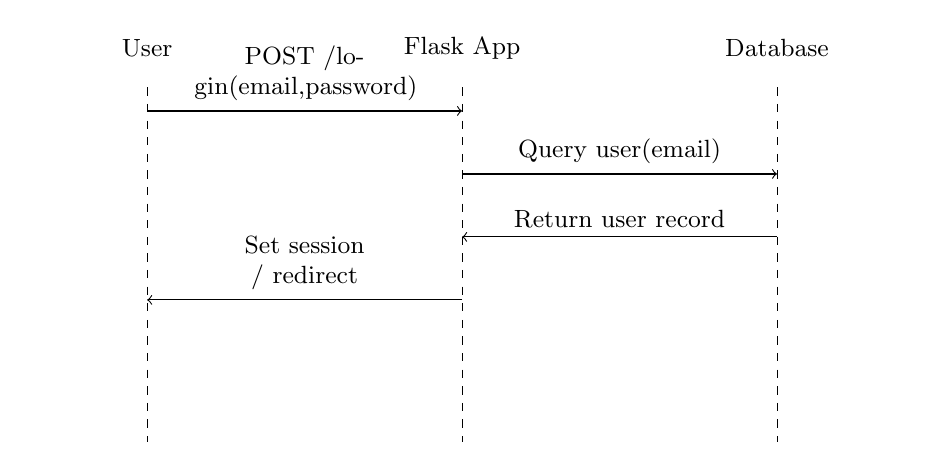
\begin{tikzpicture}[every node/.style={font=\small, text width=2.8cm, align=center}, node distance=1.5cm and 2cm]
    % Lifelines
    \node (u) at (0,0) {User};
    \node (app) at (4,0) {Flask App};
    \node (db) at (8,0) {Database};
    \draw[dashed] (0,-0.5) -- (0,-5);
    \draw[dashed] (4,-0.5) -- (4,-5);
    \draw[dashed] (8,-0.5) -- (8,-5);
    % Messages
    \draw[->] (0,-0.8) -- node[above]{POST /login(email,password)} (4,-0.8);
    \draw[->] (4,-1.6) -- node[above]{Query user(email)} (8,-1.6);
    \draw[->] (8,-2.4) -- node[above]{Return user record} (4,-2.4);
    \draw[->] (4,-3.2) -- node[above]{Set session / redirect} (0,-3.2);
\end{tikzpicture}%
}
\caption{Sequence Diagram -- User Login}
\label{fig:seqlogin}
\end{figure}

The login sequence proceeds as follows: The user sends credentials (email, password) to the Flask application via HTTP POST request. The application queries the database through SQLAlchemy to retrieve the user record. The password hash is validated using Werkzeug's check\_password\_hash function. If valid, the application creates a session and redirects to the role-specific dashboard. If invalid, an error response is returned.

%%%%%%%%%%%%%%%%%%%%%%%%%%%%%%%%%%%%%%%%%%%%%%%%%%%%%%
\subsubsection{Sequence Diagram -- Feedback Submission}

\begin{figure}[H]
\centering
\resizebox{0.9\textwidth}{!}{%
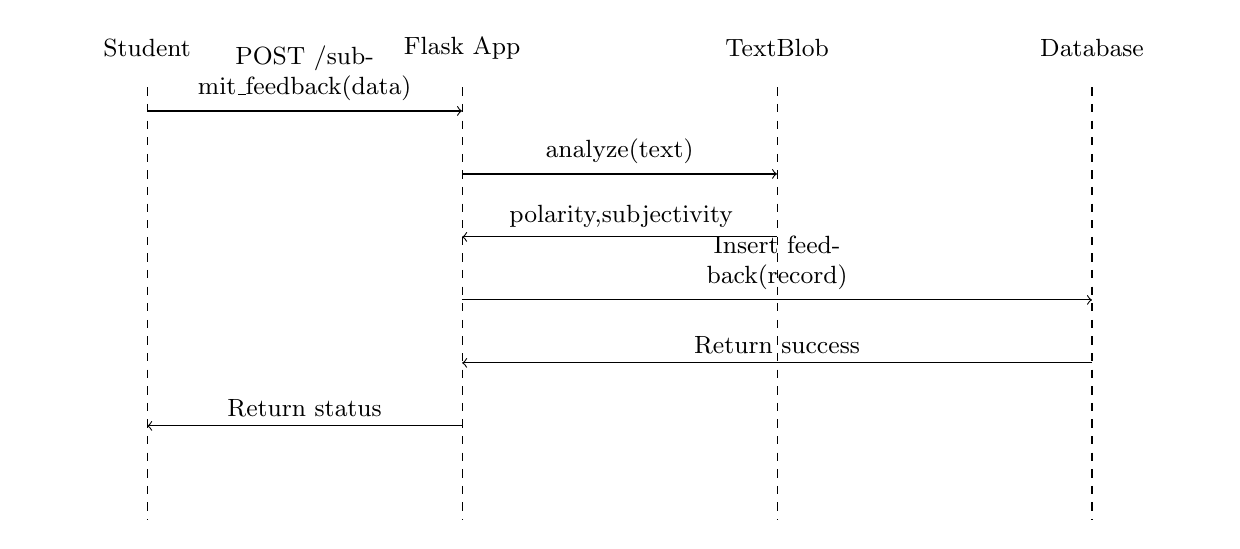
\begin{tikzpicture}[every node/.style={font=\small, text width=2.8cm, align=center}, node distance=1.5cm and 2cm]
    \node (stu) at (0,0) {Student};
    \node (app) at (4,0) {Flask App};
    \node (tb) at (8,0) {TextBlob};
    \node (db) at (12,0) {Database};
    \draw[dashed] (0,-0.5) -- (0,-6);
    \draw[dashed] (4,-0.5) -- (4,-6);
    \draw[dashed] (8,-0.5) -- (8,-6);
    \draw[dashed] (12,-0.5) -- (12,-6);
    \draw[->] (0,-0.8) -- node[above]{POST /submit\_feedback(data)} (4,-0.8);
    \draw[->] (4,-1.6) -- node[above]{analyze(text)} (8,-1.6);
    \draw[->] (8,-2.4) -- node[above]{polarity,subjectivity} (4,-2.4);
    \draw[->] (4,-3.2) -- node[above]{Insert feedback(record)} (12,-3.2);
    \draw[->] (12,-4.0) -- node[above]{Return success} (4,-4.0);
    \draw[->] (4,-4.8) -- node[above]{Return status} (0,-4.8);
\end{tikzpicture}%
}
\caption{Sequence Diagram -- Feedback Submission and Analysis}
\label{fig:seqfeedback}
\end{figure}

The feedback submission sequence involves: Student submits feedback form data via AJAX POST request. Flask application validates input fields. TextBlob library processes feedback text to calculate polarity and subjectivity scores. The system classifies sentiment based on polarity thresholds. AI suggestion engine performs keyword analysis and generates recommendations. Feedback record is stored in database via SQLAlchemy. Email notification is sent through Gmail SMTP. JSON response with sentiment result and suggestions is returned to the student's browser.

%%%%%%%%%%%%%%%%%%%%%%%%%%%%%%%%%%%%%%%%%%%%%%%%%%%%%%
\subsection{State Transition Diagrams}

\begin{figure}[H]
\centering
\resizebox{0.9\textwidth}{!}{%
\begin{tikzpicture}[every node/.style={font=\small, text width=2.5cm, align=center}, node distance=1.5cm and 2cm]
    \node[circle, draw, fill=black, minimum size=6pt] (start) {};
    \node[draw, rounded corners, right=of start, minimum width=3.5cm] (pending) {Feedback Window Open};
    \node[draw, rounded corners, below=of pending, minimum width=3.5cm] (submitted) {Submitted};
    \node[draw, rounded corners, below=of submitted, minimum width=3.5cm] (analyzed) {Analyzed};
    \node[draw, rounded corners, below=of analyzed, minimum width=3.5cm] (closed) {Feedback Window Closed};
    \draw[->] (start) -- (pending) node[midway, above, font=\footnotesize]{lecture end};
    \draw[->] (pending) -- (submitted) node[midway, right, font=\footnotesize]{submit};
    \draw[->] (submitted) -- (analyzed) node[midway, right, font=\footnotesize]{run analysis};
    \draw[->] (analyzed) -- (closed) node[midway, right, font=\footnotesize]{deadline};
\end{tikzpicture}%
}
\caption{State Transition Diagram -- Feedback Lifecycle}
\label{fig:statetransition}
\end{figure}

The state transition diagram illustrates the lifecycle of a feedback entry in the system:

\begin{itemize}
    \item \textbf{Lecture Session States}: Scheduled $\rightarrow$ In Progress $\rightarrow$ Completed $\rightarrow$ Feedback Window Open $\rightarrow$ Feedback Window Closed
    \item \textbf{Feedback States}: Pending (window open for student) $\rightarrow$ Submitted $\rightarrow$ Analyzed (sentiment computed) $\rightarrow$ Approved/Rejected (by admin)
    \item \textbf{User Account States}: Created $\rightarrow$ Active $\rightarrow$ Suspended $\rightarrow$ Deactivated
\end{itemize}

Transitions are triggered by user actions (lecture end, feedback submission, admin approval) and system events (sentiment analysis completion, deadline expiration).

%%%%%%%%%%%%%%%%%%%%%%%%%%%%%%%%%%%%%%%%%%%%%%%%%%%%%%
\section{Data Flow Diagrams}

Data Flow Diagrams (DFD) describe how data moves within the TechAware system. 
Different levels of DFD provide increasing detail.

\subsection{Level 1 Data Flow Diagram}

\begin{figure}[H]
\centering
\resizebox{0.9\textwidth}{!}{%
\begin{tikzpicture}[node distance=1.5cm and 2cm, every node/.style={font=\small, text width=2.6cm, align=center}]
    \node[draw, rectangle] (auth) {Authentication Module};
    \node[draw, rectangle, right=of auth] (acad) {Academic Management};
    \node[draw, rectangle, right=of acad] (feedback) {Feedback Processing};
    \node[draw, rectangle, below=of feedback] (notify) {Notification Module};
    \node[draw, rectangle, below=of acad] (report) {Reporting Module};
    \node[draw, rectangle, minimum width=2.8cm, minimum height=1cm, below=of auth] (db) {Database Store};
    \draw ($(db.north west)+(0.12,-0.12)$) -- ($(db.south west)+(0.12,0.12)$);
    \draw ($(db.north west)+(0.30,-0.12)$) -- ($(db.south west)+(0.30,0.12)$);
    \draw[->] (auth) -- node[midway, above, font=\footnotesize]{credentials} (acad);
    \draw[->] (acad) -- node[midway, above, font=\footnotesize]{course/batch data} (feedback);
    \draw[->] (feedback) -- node[midway, right, font=\footnotesize]{feedback records} (db);
    \draw[->] (feedback) -- node[midway, right, font=\footnotesize]{alerts} (notify);
    \draw[->] (report) -- node[midway, left, font=\footnotesize]{generate PDF} (db);
\end{tikzpicture}%
}
\caption{Level 1 DFD of TechAware AI-Based Feedback System}
\label{fig:dfd1}
\end{figure}

The Level 1 DFD decomposes the system into the following major sub-processes:

\begin{itemize}
    \item \textbf{Authentication Module}: Processes login requests, validates credentials, manages sessions.
    \item \textbf{Academic Management Module}: Handles CRUD operations for departments, batches, sections, courses, and teachers.
    \item \textbf{Feedback Processing Module}: Receives student feedback, triggers sentiment analysis, generates AI suggestions.
    \item \textbf{Notification Module}: Sends email notifications to teachers and batch advisors.
    \item \textbf{Reporting Module}: Generates PDF reports and dashboard analytics.
    \item \textbf{Database Store}: Central data store for all system entities.
\end{itemize}

Data flows connect external actors to processing modules and data stores, maintaining consistency with the context diagram.

%%%%%%%%%%%%%%%%%%%%%%%%%%%%%%%%%%%%%%%%%%%%%%%%%%%%%%
\subsection{Level 2 Data Flow Diagram}

The Level 2 DFD further decomposes the Feedback Processing Module from Level 1.

\begin{figure}[H]
\centering
\resizebox{0.9\textwidth}{!}{%
\begin{tikzpicture}[node distance=1.5cm and 2cm, every node/.style={font=\small}]
    \node[draw, rounded corners] (input) {Input Validation};
    \node[draw, rounded corners, right=of input] (sent) {Sentiment Analysis};
    \node[draw, rounded corners, right=of sent] (class) {Classification};
    \node[draw, rounded corners, below=of sent] (ai) {AI Suggestion Generation};
    \node[draw, rounded corners, below=of class] (store) {Data Storage};
    \draw[->] (input) -- (sent) node[midway, above, font=\footnotesize]{clean text};
    \draw[->] (sent) -- (class) node[midway, above, font=\footnotesize]{polarity};
    \draw[->] (class) -- (store) node[midway, right, font=\footnotesize]{record};
    \draw[->] (sent) -- (ai) node[midway, right, font=\footnotesize]{keywords};
    \draw[->] (ai) -- (store) node[midway, right, font=\footnotesize]{suggestions};
\end{tikzpicture}%
}
\caption{Level 2 DFD -- Feedback Processing Module}
\label{fig:dfd2}
\end{figure}

The Feedback Processing Module is decomposed into:
\begin{itemize}
    \item \textbf{Input Validation}: Validates form fields (ratings, text length, required fields).
    \item \textbf{Sentiment Analysis}: Processes feedback text through TextBlob to compute polarity and subjectivity.
    \item \textbf{Classification}: Classifies feedback as Understood (polarity $>$ 0.1), Not Understood (polarity $<$ --0.1), or Neutral.
    \item \textbf{AI Suggestion Generation}: Analyzes feedback text for keywords and generates context-specific teaching improvement suggestions.
    \item \textbf{Data Storage}: Stores complete feedback record with analysis results in the database.
\end{itemize}

%%%%%%%%%%%%%%%%%%%%%%%%%%%%%%%%%%%%%%%%%%%%%%%%%%%%%%
\section{Data Design}

This section describes how data is structured, stored, and managed in the TechAware system.

The system uses SQLite relational database managed through SQLAlchemy ORM. The database follows normalized schema design (3NF) to minimize redundancy and ensure data integrity. Indexing is applied on frequently queried attributes (registration\_number, session\_id, teacher\_id) to improve query performance. Security mechanisms include password hashing using bcrypt, role-based access control at the application level, and input validation for all database operations.

%%%%%%%%%%%%%%%%%%%%%%%%%%%%%%%%%%%%%%%%%%%%%%%%%%%%%%
\subsection{Entity Relationship Diagram (ERD)}

The Entity Relationship Diagram follows traditional Chen notation where entities are represented as rectangles, attributes as ovals (with primary keys underlined), and relationships as diamonds with cardinality labels.

\begin{figure}[H]
\centering
\resizebox{\textwidth}{!}{%
% Traditional Chen-style ER Diagram for TechAware System
% Uses: Rectangles (Entities), Ovals (Attributes), Diamonds (Relationships)

\begin{tikzpicture}[
    entity/.style={rectangle, draw=blue!70, fill=blue!8, thick, minimum width=3.0cm, minimum height=1.1cm, font=\small\bfseries, align=center, text width=3cm},
    attribute/.style={ellipse, draw=black!60, fill=yellow!10, thin, minimum width=1.6cm, minimum height=0.7cm, font=\small, inner sep=2pt, align=center, text width=2.2cm},
    key/.style={ellipse, draw=black!60, fill=yellow!10, thin, minimum width=1.6cm, minimum height=0.7cm, font=\small\bfseries, inner sep=2pt, align=center, text width=2.2cm},
    relationship/.style={diamond, draw=red!70, fill=red!8, thick, minimum width=2.2cm, minimum height=1.0cm, font=\small\bfseries, inner sep=2pt, aspect=2},
    every edge/.style={draw, thick},
    cardlabel/.style={font=\small, fill=white, inner sep=1pt},
    >=Latex,
    node distance=2.8cm and 3.5cm
]

% ===== ENTITIES =====

% Department - top center
\node[entity] (dept) at (0, 10) {Department};

% User Table - top right
\node[entity] (user) at (10, 10) {User};

% Batch - left
\node[entity] (batch) at (-4, 6) {Batch};

% Course - right
\node[entity] (course) at (4, 6) {Course};

% Section - center
\node[entity] (section) at (0, 4.5) {Section};

% Teacher - left
\node[entity] (teacher) at (-6, 2.5) {Teacher};

% Student - right
\node[entity] (student) at (6, 2.5) {Student};

% Batch Subject - far left
\node[entity] (bsub) at (-8, -1) {Batch\_Subject};

% Course Teacher - left
\node[entity] (ctch) at (-3, -1) {Course\_Teacher};

% Timetable - center
\node[entity] (timetable) at (3, -1) {Timetable};

% Feedback - bottom center
\node[entity] (feedback) at (0, -4.5) {Feedback};

% Student Course - far right
\node[entity] (scourse) at (9, -1) {Student\_Course};


% ===== DEPARTMENT ATTRIBUTES =====
\node[key] (dept_id) [above left=0.6cm and 1.0cm of dept] {\underline{id}};
\node[attribute] (dept_code) [above=0.6cm of dept] {code};
\node[attribute] (dept_name) [above right=0.6cm and 1.0cm of dept] {name};
\node[attribute] (dept_desc) [left=0.9cm of dept] {description};
\node[attribute] (dept_active) [below left=0.5cm and 1.2cm of dept] {is\_active};
\draw (dept) -- (dept_id);
\draw (dept) -- (dept_code);
\draw (dept) -- (dept_name);
\draw (dept) -- (dept_desc);
\draw (dept) -- (dept_active);

% ===== USER ATTRIBUTES =====
\node[key] (user_id) [above left=0.6cm and 0.8cm of user] {\underline{id}};
\node[attribute] (user_name) [above=0.6cm of user] {username};
\node[attribute] (user_email) [above right=0.6cm and 0.8cm of user] {email};
\node[attribute] (user_pass) [right=0.9cm of user] {password\_hash};
\node[attribute] (user_role) [below right=0.5cm and 0.8cm of user] {role};
\node[attribute] (user_active) [below=0.7cm of user] {is\_active};
\draw (user) -- (user_id);
\draw (user) -- (user_name);
\draw (user) -- (user_email);
\draw (user) -- (user_pass);
\draw (user) -- (user_role);
\draw (user) -- (user_active);

% ===== BATCH ATTRIBUTES =====
\node[key] (batch_id) [above left=0.5cm and 0.9cm of batch] {\underline{id}};
\node[attribute] (batch_name) [above=0.6cm of batch] {name};
\node[attribute] (batch_year) [above right=0.5cm and 0.8cm of batch] {year};
\node[attribute] (batch_sem) [left=0.9cm of batch] {semester};
\node[attribute] (batch_dept) [below left=0.5cm and 0.9cm of batch] {dept\_id (FK)};
\draw (batch) -- (batch_id);
\draw (batch) -- (batch_name);
\draw (batch) -- (batch_year);
\draw (batch) -- (batch_sem);
\draw (batch) -- (batch_dept);

% ===== COURSE ATTRIBUTES =====
\node[key] (course_id) [above left=0.5cm and 0.8cm of course] {\underline{id}};
\node[attribute] (course_code) [above=0.6cm of course] {code};
\node[attribute] (course_name) [above right=0.5cm and 0.8cm of course] {name};
\node[attribute] (course_dept) [right=0.9cm of course] {dept\_id (FK)};
\node[attribute] (course_credit) [below right=0.5cm and 0.8cm of course] {credit\_hours};
\draw (course) -- (course_id);
\draw (course) -- (course_code);
\draw (course) -- (course_name);
\draw (course) -- (course_dept);
\draw (course) -- (course_credit);

% ===== SECTION ATTRIBUTES =====
\node[key] (sec_id) [left=0.9cm of section] {\underline{id}};
\node[attribute] (sec_name) [right=0.9cm of section] {name};
\node[attribute] (sec_batch) [below left=0.4cm and 0.9cm of section] {batch\_id (FK)};
\node[attribute] (sec_cap) [below right=0.4cm and 0.9cm of section] {capacity};
\draw (section) -- (sec_id);
\draw (section) -- (sec_name);
\draw (section) -- (sec_batch);
\draw (section) -- (sec_cap);

% ===== TEACHER ATTRIBUTES =====
\node[key] (teach_id) [above=0.6cm of teacher] {\underline{id}};
\node[attribute] (teach_name) [above left=0.5cm and 0.8cm of teacher] {name};
\node[attribute] (teach_email) [left=0.9cm of teacher] {email};
\node[attribute] (teach_emp) [below left=0.5cm and 0.8cm of teacher] {employee\_id};
\node[attribute] (teach_desig) [below=0.6cm of teacher] {designation};
\draw (teacher) -- (teach_id);
\draw (teacher) -- (teach_name);
\draw (teacher) -- (teach_email);
\draw (teacher) -- (teach_emp);
\draw (teacher) -- (teach_desig);

% ===== STUDENT ATTRIBUTES =====
\node[key] (stu_id) [above=0.6cm of student] {\underline{id}};
\node[attribute] (stu_reg) [above right=0.5cm and 0.8cm of student] {reg\_number};
\node[attribute] (stu_name) [right=0.9cm of student] {name};
\node[attribute] (stu_email) [below right=0.5cm and 0.8cm of student] {email};
\node[attribute] (stu_batch) [below=0.6cm of student] {batch\_id (FK)};
\draw (student) -- (stu_id);
\draw (student) -- (stu_reg);
\draw (student) -- (stu_name);
\draw (student) -- (stu_email);
\draw (student) -- (stu_batch);

% ===== FEEDBACK ATTRIBUTES =====
\node[key] (fb_id) [left=1.5cm of feedback] {\underline{id}};
\node[attribute] (fb_text) [below left=0.5cm and 1.3cm of feedback] {feedback\_text};
\node[attribute] (fb_sent) [below=0.6cm of feedback] {sentiment};
\node[attribute] (fb_pol) [below right=0.5cm and 1.3cm of feedback] {polarity};
\node[attribute] (fb_rating) [right=1.5cm of feedback] {rating\_overall};
\node[attribute] (fb_sug) [above right=0.5cm and 1.8cm of feedback] {suggestions};
\node[attribute] (fb_date) [above left=0.5cm and 1.8cm of feedback] {created\_at};
\draw (feedback) -- (fb_id);
\draw (feedback) -- (fb_text);
\draw (feedback) -- (fb_sent);
\draw (feedback) -- (fb_pol);
\draw (feedback) -- (fb_rating);
\draw (feedback) -- (fb_sug);
\draw (feedback) -- (fb_date);


% ===== RELATIONSHIPS (Diamonds) =====

% Department --has--> Batch
\node[relationship] (r_dept_batch) at (-2, 8) {has};
\draw (dept) -- (r_dept_batch) node[cardlabel, midway, above] {1};
\draw (r_dept_batch) -- (batch) node[cardlabel, midway, left] {N};

% Department --offers--> Course
\node[relationship] (r_dept_course) at (2, 8) {offers};
\draw (dept) -- (r_dept_course) node[cardlabel, midway, above] {1};
\draw (r_dept_course) -- (course) node[cardlabel, midway, right] {N};

% Batch --contains--> Section
\node[relationship] (r_batch_sec) at (-2, 5.2) {contains};
\draw (batch) -- (r_batch_sec) node[cardlabel, midway, above] {1};
\draw (r_batch_sec) -- (section) node[cardlabel, midway, right] {N};

% Section --enrolled_in--> Student
\node[relationship] (r_sec_stu) at (3.5, 3.5) {enrolled};
\draw (section) -- (r_sec_stu) node[cardlabel, midway, above] {1};
\draw (r_sec_stu) -- (student) node[cardlabel, midway, right] {N};

% Teacher --teaches--> Course_Teacher
\node[relationship] (r_teach_ct) at (-4.5, 0.5) {teaches};
\draw (teacher) -- (r_teach_ct) node[cardlabel, midway, left] {1};
\draw (r_teach_ct) -- (ctch) node[cardlabel, midway, left] {N};

% Batch --assigns--> Batch_Subject
\node[relationship] (r_batch_bs) at (-6, 3) {assigns};
\draw (batch) -- (r_batch_bs) node[cardlabel, midway, left] {1};
\draw (r_batch_bs) -- (bsub) node[cardlabel, midway, left] {N};

% Course --assigned--> Batch_Subject
\node[relationship] (r_course_bs) at (-5.5, 1.5) {maps};
\draw (course.west) -- (r_course_bs) node[cardlabel, midway, above] {1};
\draw (r_course_bs) -- (bsub) node[cardlabel, midway, below] {N};

% BatchSubject --maps--> Course_Teacher
\node[relationship] (r_bs_ct) at (-5.5, -1) {links};
\draw (bsub) -- (r_bs_ct) node[cardlabel, midway, above] {1};
\draw (r_bs_ct) -- (ctch) node[cardlabel, midway, above] {N};

% Student --submits--> Feedback
\node[relationship] (r_stu_fb) at (4, -2.8) {submits};
\draw (student.south) -- (r_stu_fb) node[cardlabel, midway, right] {1};
\draw (r_stu_fb) -- (feedback) node[cardlabel, midway, below] {N};

% Teacher --reviewed--> Feedback
\node[relationship] (r_teach_fb) at (-4, -2.8) {reviewed\_by};
\draw (teacher.south) -- (r_teach_fb) node[cardlabel, midway, left] {1};
\draw (r_teach_fb) -- (feedback) node[cardlabel, midway, below] {N};

% Course --receives--> Feedback
\node[relationship] (r_course_fb) at (0, -2.5) {receives};
\draw (course.south) -- ++(0,-1.5) -| (r_course_fb) node[cardlabel, near start, right] {1};
\draw (r_course_fb) -- (feedback) node[cardlabel, midway, right] {N};

% Batch --schedules--> Timetable
\node[relationship] (r_batch_tt) at (0, 0.5) {schedules};
\draw (batch.south) -- ++(0,-0.5) -| (r_batch_tt) node[cardlabel, near start, left] {1};
\draw (r_batch_tt) -- (timetable) node[cardlabel, midway, right] {N};

% Student --registered--> Student_Course
\node[relationship] (r_stu_sc) at (8, 0.7) {registers};
\draw (student) -- (r_stu_sc) node[cardlabel, midway, above] {1};
\draw (r_stu_sc) -- (scourse) node[cardlabel, midway, right] {N};

% Teacher --teaches_in--> Timetable
\node[relationship] (r_teach_tt) at (-2, -0.2) {scheduled\_by};
\draw (teacher.south east) -- (r_teach_tt) node[cardlabel, near start, above] {1};
\draw (r_teach_tt) -- (timetable.west) node[cardlabel, near end, above] {N};

\end{tikzpicture}

}
\caption{Entity Relationship Diagram of TechAware System (Traditional Chen Notation)}
\label{fig:erd}
\end{figure}

The ERD represents the logical database structure with the following key entities and relationships:

\begin{itemize}
    \item Department (1) $\rightarrow$ (N) Batch, Course, Teacher, Student
    \item Batch (1) $\rightarrow$ (N) Section, Student, Timetable
    \item Section (1) $\rightarrow$ (N) Student, Timetable
    \item Timetable (1) $\rightarrow$ (N) LectureSession
    \item LectureSession (1) $\rightarrow$ (N) Attendance, Feedback
    \item Student (1) $\rightarrow$ (N) Attendance, Feedback
    \item Teacher (1) $\rightarrow$ (N) Feedback, CourseTeacher
    \item Course (1) $\rightarrow$ (N) Feedback, BatchSubject, CourseTeacher
\end{itemize}



%%%%%%%%%%%%%%%%%%%%%%%%%%%%%%%%%%%%%%%%%%%%%%%%%%%%%%
\subsection{Database Architecture}

The TechAware system uses a Client-Server database architecture:

\begin{itemize}
    \item \textbf{Client-Server Architecture}: The Flask application server hosts both the web application and the SQLite database. Client browsers communicate with the server via HTTP/HTTPS requests.
    \item \textbf{ORM Abstraction}: SQLAlchemy provides database-agnostic access, enabling future migration to PostgreSQL or MySQL without code changes to model definitions.
    \item \textbf{Local File Storage}: SQLite database is stored as a single file (\texttt{instance/techaware.db}), simplifying deployment and backup procedures.
\end{itemize}

%%%%%%%%%%%%%%%%%%%%%%%%%%%%%%%%%%%%%%%%%%%%%%%%%%%%%%
\section{Database Schema Diagram}

\begin{figure}[H]
\centering
\resizebox{0.9\textwidth}{!}{%
\begin{tikzpicture}[node distance=1.5cm and 2cm, every node/.style={font=\small}]
    \node[draw, rectangle] (user) {User(id, email, password\_hash, role)};
    \node[draw, rectangle, right=of user] (student) {Student(id, reg\_number, batch\_id)};
    \node[draw, rectangle, right=of student] (feedback) {Feedback(id, student\_id, teacher\_id, text, sentiment)};
    \draw[-] (user) -- (student);
    \draw[-] (student) -- (feedback);
    \draw[-] (user) -- (feedback);
\end{tikzpicture}%
}
\caption{Database Schema Diagram of TechAware System}
\label{fig:dbschema}
\end{figure}

The Database Schema Diagram represents the physical database implementation structure showing actual table definitions, column names, data types, and foreign key relationships across all 12 system tables.

The schema supports data integrity through primary key constraints, foreign key relationships, and unique constraints (e.g., unique batch-section combination, unique batch-course assignment). Efficient querying is achieved through indexing on frequently accessed columns. The normalized design (3NF) eliminates data redundancy while maintaining referential integrity.

%%%%%%%%%%%%%%%%%%%%%%%%%%%%%%%%%%%%%%%%%%%%%%%%%%%%%%
\subsection{Data Dictionary}

The Data Dictionary defines the structure of key data elements in the system.

%%%%%%%%%%%%%%%%%%%%%%%%%%%%%%%%%%%%%%%%%%%%%%%%%%%%%%
\begin{table}[H]
\centering
\caption{Data Dictionary -- User Table}
\begin{tabularx}{\textwidth}{|p{3cm}|p{2cm}|p{2cm}|X|}
\hline
\textbf{Field Name} & \textbf{Type} & \textbf{Size} & \textbf{Description} \\
\hline
id & INT & 11 & Primary key, unique identifier for each user \\
\hline
username & VARCHAR & 80 & Unique username for login \\
\hline
email & VARCHAR & 120 & Registered email address (unique) \\
\hline
password\_hash & VARCHAR & 255 & bcrypt-hashed password \\
\hline
role & VARCHAR & 20 & User role (admin, teacher, student, batch\_advisor) \\
\hline
created\_at & DATETIME & -- & Account creation timestamp \\
\hline
is\_active & BOOLEAN & -- & Account active status (default: True) \\
\hline
\end{tabularx}
\end{table}

\begin{table}[H]
\centering
\caption{Data Dictionary -- Feedback Table}
\begin{tabularx}{\textwidth}{|p{3cm}|p{2cm}|p{2cm}|X|}
\hline
\textbf{Field Name} & \textbf{Type} & \textbf{Size} & \textbf{Description} \\
\hline
id & INT & 11 & Primary key, unique feedback identifier \\
\hline
student\_id & INT & 11 & Foreign key referencing Students table \\
\hline
student\_name & VARCHAR & 100 & Name of the student submitting feedback \\
\hline
feedback\_text & TEXT & -- & Free-text feedback content \\
\hline
sentiment & VARCHAR & 50 & Classified sentiment (Understood/Not Understood/Neutral) \\
\hline
polarity & FLOAT & -- & TextBlob polarity score (--1.0 to +1.0) \\
\hline
subjectivity & FLOAT & -- & TextBlob subjectivity score (0.0 to 1.0) \\
\hline
rating\_overall & INT & 1 & Overall satisfaction rating (1--5) \\
\hline
suggestions & TEXT & -- & JSON array of AI-generated suggestions \\
\hline
submitted\_at & DATETIME & -- & Feedback submission timestamp \\
\hline
status & VARCHAR & 20 & Approval status (submitted/approved/rejected) \\
\hline
\end{tabularx}
\end{table}

%%%%%%%%%%%%%%%%%%%%%%%%%%%%%%%%%%%%%%%%%%%%%%%%%%%%%%
%===========================================================
\section{Database Tables / Collections}
%===========================================================

This section describes the logical database design of the system. It presents the major relational tables used in the TechAware system. The database structure is designed to ensure data consistency, integrity, security, and scalability.

Each table includes primary keys, relationships, and major attributes relevant to system functionality.



%%%%%%%%%%%%%%%%%%%%%%%%%%%%%%%%%%%%%%%%%%%%%%%%%%%%%%
\subsection{User Table}
%%%%%%%%%%%%%%%%%%%%%%%%%%%%%%%%%%%%%%%%%%%%%%%%%%%%%%

The User table stores authentication credentials and role information for all system users. It supports role-based access control with four user types: admin, teacher, student, and batch\_advisor.

\textbf{Description:}
\begin{itemize}
    \item Primary Key: \texttt{id}
    \item Relationships: Users are associated with specific portals based on their role attribute.
    \item Authentication Attributes: Username, email, password hash, role, account status.
\end{itemize}

\begin{table}[H]
\centering
\caption{User Table Structure}

\begin{tabularx}{\textwidth}{|p{3cm}|p{3cm}|p{3cm}|X|}
\hline
\textbf{Field Name} & \textbf{Data Type} & \textbf{Constraint} & \textbf{Description} \\
\hline
id & INTEGER & Primary Key & Auto-incremented unique identifier \\
\hline
username & VARCHAR(80) & Unique, Not Null & Login username \\
\hline
email & VARCHAR(120) & Unique, Not Null & User email address \\
\hline
password\_hash & VARCHAR(255) & Not Null & bcrypt-hashed password \\
\hline
role & VARCHAR(20) & Not Null & User role (admin/teacher/student/batch\_advisor) \\
\hline
created\_at & DATETIME & Default Current & Account creation timestamp \\
\hline
is\_active & BOOLEAN & Default True & Account active/inactive status \\
\hline
\end{tabularx}

\end{table}



%%%%%%%%%%%%%%%%%%%%%%%%%%%%%%%%%%%%%%%%%%%%%%%%%%%%%%
\subsection{Core Data Tables}
%%%%%%%%%%%%%%%%%%%%%%%%%%%%%%%%%%%%%%%%%%%%%%%%%%%%%%

This subsection describes the domain-specific core data tables that store primary operational data.

\textbf{Feedback Table:}
\begin{itemize}
    \item Stores all student feedback submissions with ratings, text content, sentiment analysis results, and AI suggestions.
    \item Links to Student, Course, Teacher, and LectureSession tables through foreign keys.
    \item Includes approval workflow fields (status, approved\_at, approved\_by).
\end{itemize}

\textbf{Department Table:}
\begin{itemize}
    \item Stores academic department information (code, name, description).
    \item Parent entity for Batch, Student, Teacher, and Course relationships.
\end{itemize}

\textbf{Student Table:}
\begin{itemize}
    \item Stores student records with registration number, name, email, batch, section, and department associations.
    \item Includes authentication fields (password hash) for student portal login.
    \item Has one-to-many relationships with Feedback and Attendance.
\end{itemize}

\textbf{Timetable Table:}
\begin{itemize}
    \item Stores lecture schedule entries linking course, teacher, section, batch, day, time slot, and room.
    \item Used to auto-generate LectureSession records for attendance and feedback tracking.
\end{itemize}



%%%%%%%%%%%%%%%%%%%%%%%%%%%%%%%%%%%%%%%%%%%%%%%%%%%%%%
\subsection{Relationships Between Tables}
%%%%%%%%%%%%%%%%%%%%%%%%%%%%%%%%%%%%%%%%%%%%%%%%%%%%%%

Database relationships define how data entities are connected within the TechAware system.

\begin{itemize}
    \item \textbf{One-to-Many (1:N):} One Department has many Batches, Courses, Teachers, and Students.
    \item \textbf{One-to-Many (1:N):} One Batch has many Sections; one Section has many Students.
    \item \textbf{One-to-Many (1:N):} One Student generates multiple Feedback submissions and Attendance records.
    \item \textbf{Many-to-Many (M:N):} Courses are assigned to Batches through the BatchSubject junction table. Teachers are assigned to Course-Section combinations through the CourseTeacher junction table.
\end{itemize}



%%%%%%%%%%%%%%%%%%%%%%%%%%%%%%%%%%%%%%%%%%%%%%%%%%%%%%
\subsection{Security and Data Integrity}
%%%%%%%%%%%%%%%%%%%%%%%%%%%%%%%%%%%%%%%%%%%%%%%%%%%%%%

To ensure confidentiality and integrity of stored data, the following measures are implemented:

\begin{itemize}
    \item Password Encryption using bcrypt hashing algorithm through Werkzeug's generate\_password\_hash and check\_password\_hash functions.
    \item Role-Based Access Control (RBAC) restricting user access to role-appropriate portals and API endpoints.
    \item Input validation and constraint enforcement at both application and database levels (Not Null, Unique, Foreign Key constraints).
    \item Secure communication using HTTPS recommended for production deployment.
    \item CSRF protection to prevent cross-site request forgery attacks.
\end{itemize}



%%%%%%%%%%%%%%%%%%%%%%%%%%%%%%%%%%%%%%%%%%%%%%%%%%%%%%
\subsection{Scalability Considerations}
%%%%%%%%%%%%%%%%%%%%%%%%%%%%%%%%%%%%%%%%%%%%%%%%%%%%%%

The database design incorporates scalability mechanisms to support future growth.

\begin{itemize}
    \item Database migration from SQLite to PostgreSQL or MySQL is supported through SQLAlchemy ORM abstraction without code changes to model definitions.
    \item Indexing on frequently queried attributes (registration\_number, session\_id, teacher\_id, feedback timestamp) improves query performance.
    \item Modular model design allows addition of new entities (e.g., Notification, SystemConfig) without restructuring existing tables.
    \item Cascade delete operations maintain referential integrity during entity removal.
    \item Lazy loading of relationships optimizes memory usage for queries with large result sets.
\end{itemize}


%%%%%%%%%%%%%%%%%%%%%%%%%%%%%%%%%%%%%%%%%%%%%%%%%%%%%%
\section{Chapter Summary}
%%%%%%%%%%%%%%%%%%%%%%%%%%%%%%%%%%%%%%%%%%%%%%%%%%%%%%

This chapter presented the comprehensive software design of the TechAware AI-Based Feedback System. It translated the functional and non-functional requirements identified in Chapter 3 into structured architectural, behavioral, and data models.

The Layered Architecture design methodology and Agile software process model were justified to ensure systematic development and maintainability. A high-level system overview was provided through the context diagram, and the three-tier architectural design was illustrated, clearly showing the separation between presentation, application, and data layers.

Detailed UML models including activity diagrams for three core modules, class diagram showing 12 system classes with relationships, sequence diagrams for user login and feedback submission workflows, and state transition diagrams for the feedback lifecycle were developed. Data flow diagrams (Level 1 and Level 2) were constructed to represent internal data movement across system components.

The chapter further elaborated the database design through the Entity Relationship Diagram, database schema diagram, data dictionaries for User and Feedback tables, and detailed descriptions of core database tables. Relationships between entities, security measures, and scalability considerations were also documented.

Overall, this chapter establishes the technical blueprint that guides the implementation phase discussed in the next chapter.
